% Copyright (c) 2014,2016 Casper Ti. Vector
% Public domain.

\chapter{区块链的实名交易监督系统實作}

為了驗證和證明所提議的BRTMS用於比特幣支付收款監督的可行性和有效性,我們將其運行在用於商家商品管理和維護的Java應用程序的SMIMSS子系統,用於商家職員的運行在Android App上的SMCTSS以及運行在App上的用於客戶的CMPTSS。
如圖\ref{fig5}所示,SMIMSS Java應用程序可以幫助商家登錄到系統或創建一個新帳戶。 授權商戶成功登錄系統後,商家可以插入或更新產品列表,如圖\ref{fig6}所示。實施的SMIMSS Java應用程序執行前面部分中所述的功能。

\begin{figure}[h]
	\centering
	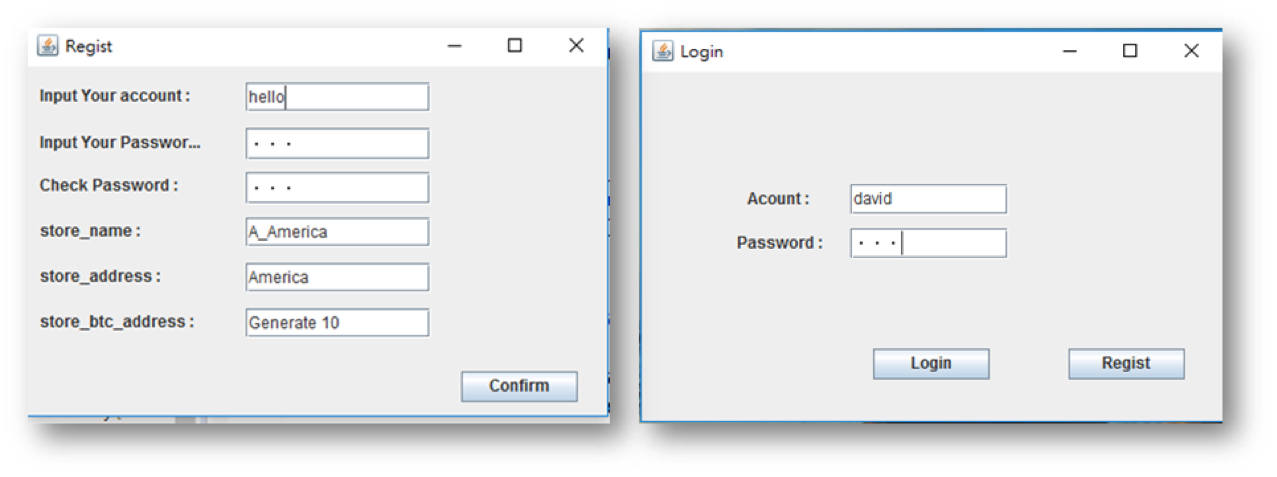
\includegraphics[width = 0.9\textwidth]{fig5.png}
	\caption{SMIMSS的Java應用程序的註冊和登錄界面}\label{fig5}
\end{figure}

\begin{figure}[h]
	\centering
	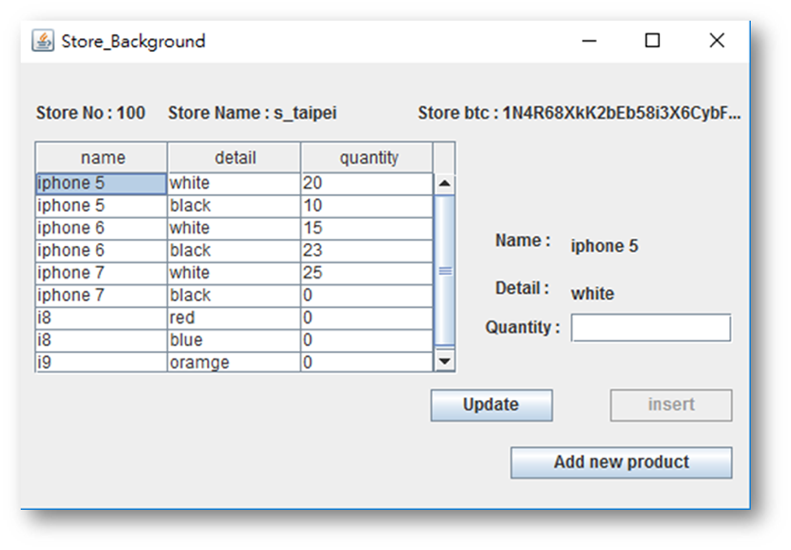
\includegraphics[width = 0.6\textwidth]{fig6.png}
	\caption{在SMIMSS中插入或更新授權商家的產品目錄}\label{fig6}
\end{figure}

商戶的產品信息可以通過RFID標籤掃描,存儲到雲端數據庫中,商戶店員可以使用我們實現的SMCTSS安卓客戶端,啟用NFC監聽器,從購物車中的客戶購買產品中讀取RFID標籤信息。 在如圖\ref{fig7}所示的第一項活動中,商家職員必須登錄才能獲得授權訪問SMCTSS功能。 然後,在第二項活動中,SMCTSS應用程序可以通過使用SMIMSS中應用的雲數據庫檢查產品RFID標籤信息並將其展示給客戶,從而將掃描的產品列入購物車。 在圖\ref{fig7}的第三項活動中,顧客可以要求店員取消購買物品以確認最終購買。 最後,SMCTSS應用程序將自動使用比特幣測試網絡幫助店員確認發布此密碼貨幣交易的收款人地址,如圖\ref{fig7}的第4項活動所示。    

\begin{figure}[h]
	\centering
	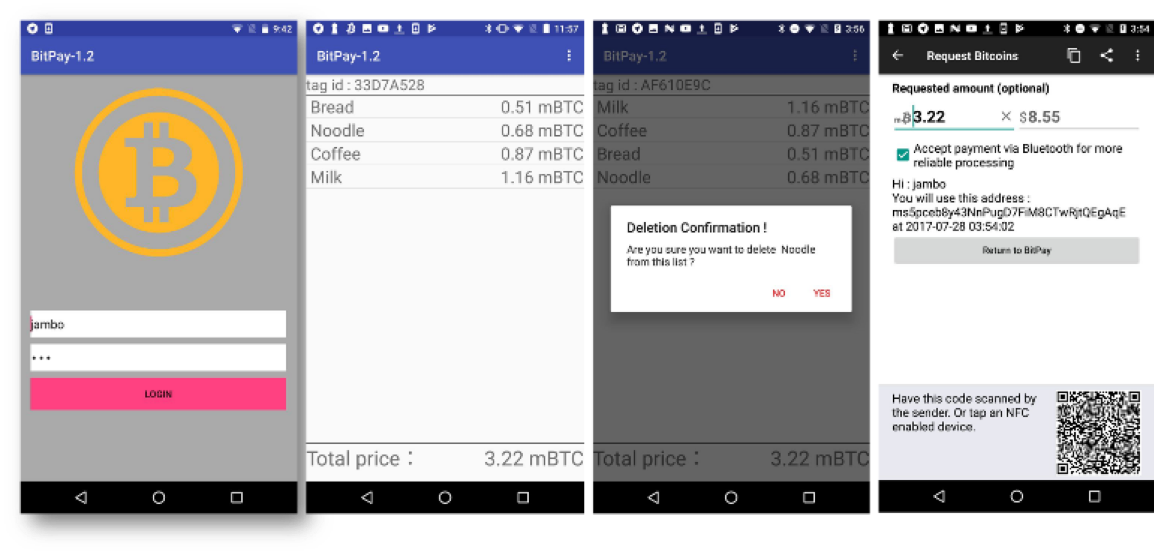
\includegraphics[width = 1\textwidth]{fig7.png}
	\caption{登錄、等待結帳的商品、刪除商品及支付確認}\label{fig7}
\end{figure}

同時,客戶將使用與SMCTSS App相對應的CMPTSS Android App通過比特幣密碼貨幣完成採購產品交易。 如圖\ref{fig8}所示,第一個活動表示顧客確認購買產品創建交易數據庫的交易清單,第二個活動顯示包括金額和付款人比特幣地址在內的付款確認,第三個活動顯示交易歷史記錄 的交易作為買方甚至是賣方,最後在第四項活動中顯示了該筆交易詳細採購產品的發票。    

\begin{figure}[h]
	\centering
	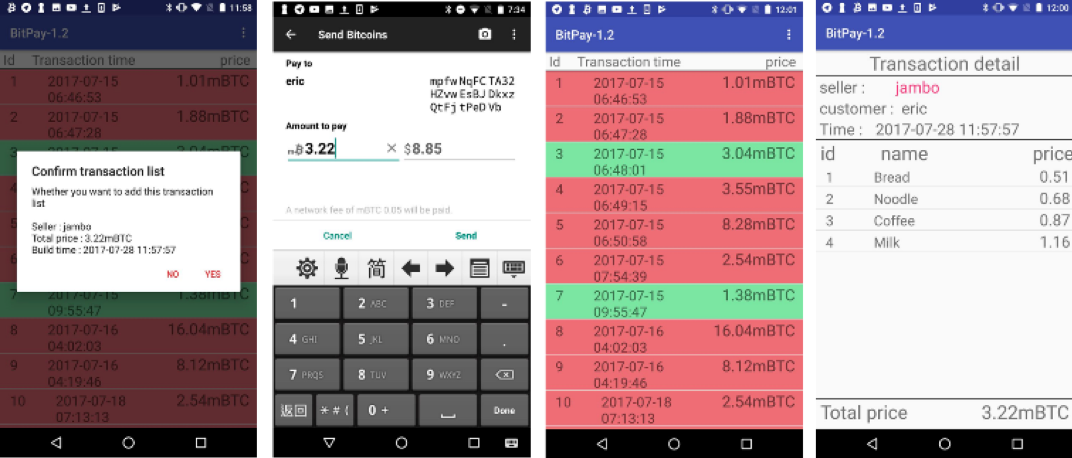
\includegraphics[width = 1\textwidth]{fig8.png}
	\caption{在CMPTSS App中,交易确认,付款确认、交易历史纪录和发票}\label{fig8}
\end{figure}